%%% LaTeX Template: Article/Thesis/etc. with colored headings and special fonts
%%%
%%% Source: http://www.howtotex.com/
%%% Feel free to distribute this template, but please keep to referal to http://www.howtotex.com/ here.
%%% February 2011
%%%
%%% Modified October 2015 by CDM

%%%  Preamble
\documentclass[11pt,letterpaper]{article}
\usepackage[margin=1.0in]{geometry}
\usepackage[T1]{fontenc}
\usepackage[bitstream-charter]{mathdesign}
\usepackage[latin1]{inputenc}					
\usepackage{amsmath}						
\usepackage{xcolor}
\usepackage{cite}
\usepackage{hyphenat}
\usepackage{graphicx}
\usepackage{float}
\usepackage{subfigure}
\usepackage{sectsty}
\usepackage[compact]{titlesec} 
\usepackage[tablegrid]{vhistory}
\allsectionsfont{\color{accentcolor}\scshape\selectfont}

%%% Definitions
\definecolor{accentcolor}{rgb}{0.0,0.0,0.5} 
\newcommand{\teamname}{TrafficNetPeons}
\newcommand{\productname}{Product Name: TBD}
\newcommand{\coursename}{CSE 4316: Senior Design I}
\newcommand{\semester}{Spring 2016}
\newcommand{\docname}{System Requirements Specification}
\newcommand{\department}{Department of Computer Science \& Engineering}
\newcommand{\university}{The University of Texas at Arlington}
\newcommand{\authors}{Peyton Casper \\ Rabin Dhoubonjar \\ Kyle Edelmann \\ Jose Hernandez \\ Ruchitha Thalakola}

%%% Headers and footers
\usepackage{fancyhdr}
	\pagestyle{fancy}						% Enabling the custom headers/footers
\usepackage{lastpage}	
	% Header (empty)
	\lhead{}
	\chead{}
	\rhead{}
	% Footer
	\lfoot{\footnotesize \teamname \ - \semester}
	\cfoot{}
	\rfoot{\footnotesize page \thepage\ of \pageref{LastPage}}	% "Page 1 of 2"
	\renewcommand{\headrulewidth}{0.0pt}
	\renewcommand{\footrulewidth}{0.4pt}

%%% Change the abstract environment
\usepackage[runin]{abstract}			% runin option for a run-in title
%\setlength\absleftindent{30pt}			% left margin
%\setlength\absrightindent{30pt}		% right margin
\abslabeldelim{\quad}	
\setlength{\abstitleskip}{-10pt}
\renewcommand{\abstractname}{}
\renewcommand{\abstracttextfont}{\color{accentcolor} \small \slshape}	% slanted text

%%% Start of the document
\begin{document}

%%% Cover sheet
{{\centering \huge \color{accentcolor} \sc \textbf{\department \\ \university} \par}
\vspace{1 in}
{\centering \huge \color{accentcolor} \sc \textbf{\docname \\ \coursename \\ \semester} \par}
\vspace{0.5 in}
\begin{figure}[h!]
	\centering
   	
\includegraphics[width=0.45\textwidth]{images/tp_logo.jpg}
\end{figure}
\vspace{0.5 in}
{\centering \huge \color{accentcolor} \sc \textbf{\teamname \\ \productname} \par}
\vspace{0.5 in}
{\centering \large \sc \textbf{\authors} \par}
\newpage

%\vspace{1 in}
%\centerline{January 13th, 2012}
%\newpage

%%% Revision History
\begin{versionhistory}
  	\vhEntry{0.1}{03.01.2016}{PC}{Document Creation}
  	\vhEntry{0.2}{03.09.2016}{PC|JH|RT|RD|KE}{Initial Draft Complete}
  	\vhEntry{0.3}{03.10.2016}{PC|JH|RT|RD|KE}{Updated Draft}
  	\vhEntry{1.0}{03.11.2016}{PC|JH|RT|RD|KE}{Document Release}
\end{versionhistory}
\newpage

%%% Table of contents
\setcounter{tocdepth}{2}
\tableofcontents
\newpage

%%% List of figures and tables (optional)
\listoffigures
%\listoftables
\newpage

\section{Product Concept}
This section provides a high-level statement of your product concept - what it is intended to do and how it is intended to be used. Include in this header paragraph, a brief synopsis of what is described here. For example, this header paragraph might say something like: "This section describes the purpose, use and intended user audience for the X product. X is a system that performs Y. Users of X will be able to Z..."

\subsection{Purpose and Use}
This is where you describe in a brief, yet clear and concise, manner what your product should do and how you expect it should be used.

\subsection{Intended Audience}
This is where you describe the intended audience(s) of your product. If this product were to be made available publicly or commercially, who would purchase or use it? Is the product designed for a particular customer, or an overall class of customers? Is it intended for general use, or is it a specific component of a more complex system?

\begin{figure}[h!]
	\centering
   	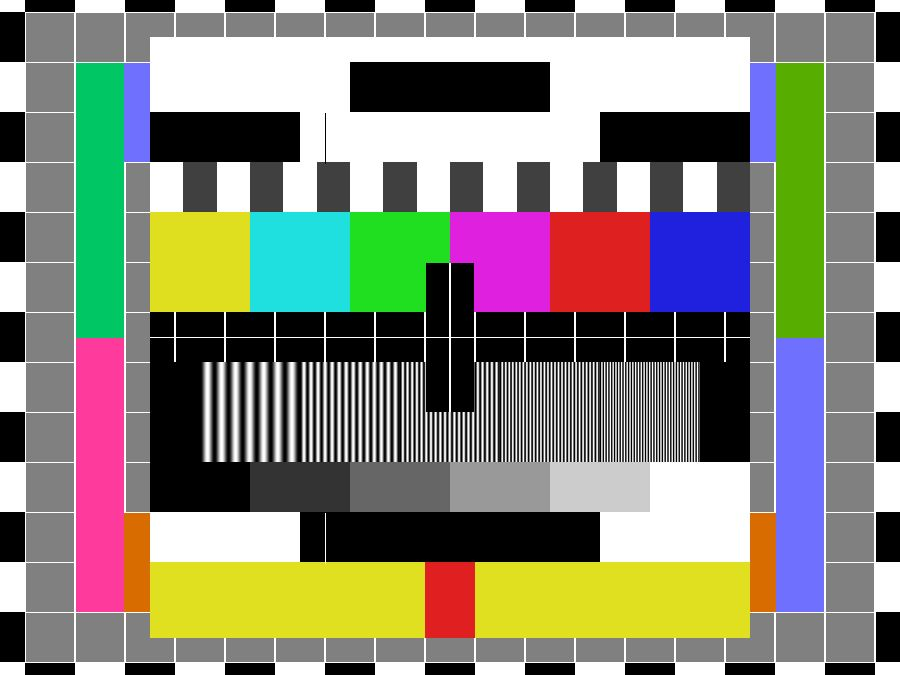
\includegraphics[width=0.60\textwidth]{images/test_image}
    \caption{X conceptual drawing}
\end{figure}

\newpage
\section{Product Description}
This section provides a description of your product and defines it's primary features and functions. The purpose is to give the document reader/reviewer enough information about the product to allow them to easily follow the specification of requirements found in the remainder of the document. Your header for this section should introduce the section with a brief statement such as: "This section provides the reader with an overview of X. The primary operational aspects of the product, from the perspective of end users, maintainers and administrators, are defined here. The key features and functions found in the product, as well as critical user interactions and user interfaces are described in detail." Using words, and pictures or graphics where possible, specify the following:

\subsection{Features \& Functions}
What the product does and does not do. Specify in words what it looks like, referring to a conceptual diagram/graphic (Figure X).  Define the principle parts/components of the product. Specify the elements in the diagram/graphic that are part(s) of this product as well as any associated external elements (e.g., the Internet, an external web server, a GPS satellite, etc.)

\subsection{External Inputs \& Outputs}
Describe critical external data flows. What does your product require/expect to receive from end users or external systems (inputs), and what is expected to be created by your product for consumption by end users or external systems (outputs)? In other words, specify here all data/information to flow into and out of your systems. A table works best here, with rows for each critical data element, and columns for name, description and use.

\subsection{Product Interfaces}
Specify what all operational (visible) interfaces look like to your end-user, administrator, maintainer, etc. Show sample/mocked-up screen shots, graphics of buttons, panels, etc. Refer to the critical external inputs and outputs described in the paragraph above.

\newpage
\section{Customer Requirements}
Include a header paragraph specific to your product here. Customer requirements are those required features and functions specified for and by the intended audience for this product. This section establishes, clearly and concisely, the "look and feel" of the product, what each potential end-user should expect the product do and/or not do. Each requirement specified in this section is associated with a specific customer need that will be satisfied. In general Customer Requirements are the directly observable features and functions of the product that will be encountered by its users. Requirements specified in this section are created with, and must not be changed without, specific agreement of the intended customer/user/sponsor.

\subsection{Requirement Name}
\subsubsection{Description}
A detailed description of the feature/function that satisfies the requirement. For example: \textit{The box will be slate blue. This specific color is required in order to ensure that the box matches other similar boxes in the Box Systems Premium line of products. Slate blue is specified as \#007FFF, using six-digit hexadecimal color specification.} It is acceptable and advisable to include drawings/graphics in the description if it aids understanding of the requirement.
\subsubsection{Source}
The source of the requirement (e.g. customer, sponsor, specified team member (by name), federal regulation, local laws, CSE Senior Design project specifications, etc.)
\subsubsection{Constraints}
A detailed description of constraints on satisfying the requirement (e.g. one such constraint might be: \textit{The specified color must be commercially available in paint capable of adhering to the material of which the box is manufactured. (See customer requirement 3.x for production material specification.)}
\subsubsection{Standards}
A detailed description of any specific standards that apply to this requirement (e.g. \textit{NSTM standard xx.xxx.x. color specifications \cite{Rubin2012}}.)
\subsubsection{Priority}
The priority of this requirement relative to other specified requirements. Use the following priorities:
\begin{itemize}
\item Critical (must have or product is a failure)
\item High (very important to customer acceptance, desirability)
\item Moderate (should have for proper product functionality);
\item Low (nice to have, will include if time/resource permits)
\item Future (not feasible in this version of the product, but should be considered for a future release).
\end{itemize}

\subsection{Requirement Name}
\subsubsection{Description}
Detailed requirement description...
\subsubsection{Source}
Source
\subsubsection{Constraints}
Detailed description of applicable constraints...
\subsubsection{Standards}
List of applicable standards
\subsubsection{Priority}
Priority

\newpage
\section{Packaging Requirements}
Include a header paragraph here. Packaging requirements are those requirements that identify how the delivered product will be packaged for delivery to the end-user; or how it will "look" when finished and delivered. For example, you might specify that the software required for operation will be pre-loaded on the hard drive, delivered on CD/DVD, or available via download. Software might be customer installable, or not, etc. Hardware components could be all in a single package, provided as a "bag of parts" to be assembled/installed by the user, painted a certain color, logos affixed, etc. Care should be taken not to duplicate requirements found in other sections of this document.

\subsection{Requirement Name}
\subsubsection{Description}
Detailed requirement description...
\subsubsection{Source}
Source
\subsubsection{Constraints}
Detailed description of applicable constraints...
\subsubsection{Standards}
List of applicable standards
\subsubsection{Priority}
Priority
\newpage
\section{Performance Requirements}
The sections will provide the information about the performance requirements that are necessary for the surveillance camera to perform at the acceptable level. The product should fulfill the certain performance criteria like zooming capacity, power consumption, tilt and rotate at certain angle, etc. 


\subsection{Power Comsumption}
\subsubsection{Description}
The camera should operate at the power of 5 watts.
\subsubsection{Source}
Traffic Net
\subsubsection{Constraints}
The low power consumption lowers the performance.
\subsubsection{Standards}
None.
\subsubsection{Priority}
High.


\subsection{Zooming Capability}
\subsubsection{Description}
The camera should be able to zoom the object by 10 times
\subsubsection{Source}
Traffic Net
\subsubsection{Constraints}
The video will not be of high quality.
\subsubsection{Standards}
None.
\subsubsection{Priority}
High

\subsection{Pixel And Frame Rates}
\subsubsection{Description}
The system shall operate at 520p at 10fps.
\subsubsection{Source}
Traffic Net
\subsubsection{Constraints}
Poor picture quality.
\subsubsection{Standards}
None.
\subsubsection{Priority}
High

\subsection{Operating Temperature}
\subsubsection{Description}
The camera should operate between the temperature of range -20 C and 80 C.
\subsubsection{Source}
Traffic Net
\subsubsection{Constraints}
Performance of the camera.
\subsubsection{Standards}
None.
\subsubsection{Priority}
High


\subsection{Tilt And Rotate}
\subsubsection{Description}
The camera should tilt 180 degree and rotate 360 degree.
\subsubsection{Source}
Traffic Net
\subsubsection{Constraints}
Performance of the camera.
\subsubsection{Standards}
None.
\subsubsection{Priority}
High

\newpage
\section{Safety Requirements}
This section will address safety requirements regarding the camera. It will list and describe in detail the precautions that must be taken in order to safely and properly utilize this product. Ensuring that these requirements are properly implemented will assure the safety of all individuals involved. 


\subsection{Camera Enclosure Material}
\subsubsection{Description}
The material of the camera enclosure must not contain glass. This will provide safety to all individuals from the glass that may break off due to certain weather conditions or other circumstances.
\subsubsection{Source}
CSE Senior Design project specifications
\subsubsection{Constraints}
The manufacturer must find another material that is satisfactory and enables the safety of the camera and the individuals involved during all circumstances. 
\subsubsection{Standards}
N/A
\subsubsection{Priority}
Priority 2

\subsection{Camera Interior Packaging }
\subsubsection{Description}
The pieces located inside the camera enclosure must organized and packaged in a way that prevents cuts from sharp edges or shock. This will ensure that individuals handling the product will not be injured. 
\subsubsection{Source}
CSE Senior Design project specifications
\subsubsection{Constraints}
The manufacturer must find materials and parts used to make the interior component of the camera that will not be able to injure an individual who is touching the material by cutting or shocking them.
\subsubsection{Standards}
N/A
\subsubsection{Priority}
Priority 2

\newpage
\section{Maintenance \& Support Requirements}
This section will address maintenance and support requirements for the camera. It will list and describe in detail the maintenance and support that will be necessary to amend any issues that may occur after the delivery of the product. Maintenance and support requirements regarding both hardware and software components will be provided. 

\subsection{Camera Exterior Maintenance}
\subsubsection{Description}
The exterior of the camera must undergo maintenance semiannually. The exterior must be checked for damage that can occur due to the weather and other sources. If the damage is considered to be significant, then the exterior or the entire product must be replaced. 
\subsubsection{Source}
CSE Senior Design project specifications
\subsubsection{Constraints}
The customer must have technicians available to inspect the status of the camera exterior semiannually. 
\subsubsection{Standards}
N/A
\subsubsection{Priority}
Priority 3

\subsection{Camera Interior Maintenance}
\subsubsection{Description}
The interior of the camera must undergo maintenance semiannually. The interior of the camera must be checked for damage. If the damage is considered to be significant, then certain parts or the complete component must be replaced. 
\subsubsection{Source}
CSE Senior Design project specifications
\subsubsection{Constraints}
The customer must have technicians available to inspect the status of the camera interior semiannually. 
\subsubsection{Standards}
N/A
\subsubsection{Priority}
Priority 2

\subsection{Software Maintenance}
\subsubsection{Description}
The web interface must undergo maintenance quarterly in order to assure proper functionality. All the functionalities, such as pan, tilt, and zoom must be accessed and tested to verify functionality. The technician who is responsible for the maintenance should be able to view what the camera is pointing towards clearly when testing these functionalities. 
\subsubsection{Source}
CSE Senior Design project specifications
\subsubsection{Constraints}
The customer must have experienced technicians available to check for proper functionality of the camera through the web interface. The technician must also have the user manual and source code documentation to fix any issues that occured. 
\subsubsection{Standards}
N/A
\subsubsection{Priority}
Priority 1

\newpage
\section{Other Requirements}
The following includes additional requirements that the project must have, a more detailed description of each requirement, the source, the constraits, the standards, and finally the priority of each standard that the project must have. Although the team does not have to have a final one hundred percent fully professional project by the deadline which is by the middle of March, the requirements set by TrafficNet must be complete.

\subsection{Requirement}
Some additional requirement would be to arrange all the components of the project into a professional way, cover any logos of components we might use in our project, modularity and extensibility will be required in case future enhancements might be necessary, camera has to be portable, the graphical user interface must be easy to use and work with any type of operating system.
\subsubsection{Description}
The project must be done in a professional manner which means that no hanging cables or messy implementation of components. Modularity and extensibility will be required because in case we decide to add to the project in the future, we want to know exactly what each component and connection does, so that in the future implementation will be easier. The camera does have to be portable, which means that the camera must fit on an enclosed spaced and not be to big or have cables running all over the place. The graphical user interface must be easy to use because we don't want the user to get confused about how to interact with the camera.
\subsubsection{Source}
The source comes from TrafficNet, which they gave us an idea of how the project must be implemented.
\subsubsection{Constraints}
One of the biggest contraints would be for the project to run on not more than 5W of power, which means we must make the project run on very low power and use solar panels to achieve the required amount.
\subsubsection{Standards}
Extreme low power, must have a solar panel and bettery, have pan and tilt capability, heating capability,  easy to use GUI, and 10X zoom.
\subsubsection{Priority}
The top priority would be for the system to run on extreme low power. After the top priority is achieved, the other priorities are as follows, 180 degrees pan and tilt, easy to use GUI, 10X zoom, and finally having a heating capability for extreme weather. 

\newpage
\section{Acceptance Criteria}


\newpage
\section{Use Cases}
This section is dedicated to specifying UML use cases for the user-visible features specified herein. Included in this section are details addressing administrative or maintenance support users, requirements for setup and installation procedures, as well as "customer end-user requirements."

\subsection{Warning}
Installation and servicing should be performed only by qualified and experienced technicians to conform to all local codes and to maintain your warranty.
\subsection{Setup and Installation}
\subsubsection{Scenario}
It is to be noted that supply, installation and commissioning of the system with all accessories, auxiliaries, and any item not covered in the specification but essential for proper installation, operation and maintenance of the system shall be included and executed by the vendor.
\subsubsection{Actor(s)}
The setup and installation of the camera shall be the responsibility of only a qualified vendor technician.
\subsection{Camera Operation}
\subsubsection{Scenario}
The camera shall be accessed via secured web interface.
The user shall be required to log on by entering a unique password.
A "live view" from the camera shall be displayed on the user monitor during operation. 
The view shall include pan, tilt, and lens functions (zoom, iris and focus). 
The user shall possess the ability to remotely control all viewing functionality.
The user shall possess the ability to set and clear the movement limits of the pan and tilt mechanisms so equipped.
\subsubsection{Actor(s)}
The use and operation of the camera shall be at the discretion of the administrator and/or the user.
\subsection{Adjusting the Camera}
\subsubsection{Scenario}

\subsubsection{Actor(s)}
\subsection{Routine Maintenance}

\subsubsectio{Scenario}

\subsubsection{Actor(s)}

Detailed description of applicable constraints...
\subsubsection{Standards}
List of applicable standards
\subsubsection{Priority}
Priority

\newpage
\section{Feasibility Assessment}
This section consists of an assessment of the following six components: scope analysis, research completed/remaining, technical analysis, cost analysis, resource analysis and schedule analysis in an attempt to critically analyze the feasibility of the successful fulfillment of the requirements specified herein.
\subsection{Scope Analysis}
Installation and servicing should be performed only by qualified and experienced technicians to conform to all local codes and to maintain your warranty.
\subsection{Setup and Installation}
\subsubsection{Scenario}
It is to be noted that supply, installation and commissioning of the system with all accessories, auxiliaries, and any item not covered in the specification but essential for proper installation, operation and maintenance of the system shall be included and executed by the vendor.
\subsubsection{Actor(s)}
The setup and installation of the camera shall be the responsibility of only a qualified vendor technician.
\subsection{Camera Operation}
\subsubsection{Scenario}
The camera shall be accessed via secured web interface.
The user shall be required to log on by entering a unique password.
A "live view" from the camera shall be displayed on the user monitor during operation. 
The view shall include pan, tilt, and lens functions (zoom, iris and focus). 
The user shall possess the ability to remotely control all viewing functionality.
The user shall possess the ability to set and clear the movement limits of the pan and tilt mechanisms so equipped.
\subsubsection{Actor(s)}
The use and operation of the camera shall be at the discretion of the administrator and/or user operator.
\subsection{Adjusting the Camera}
\subsubsection{Scenario}
The camera shall be adjustable in all features relating to viewing functionality remotely.
The camera shall be adjustable in all features relating to viewing functionality manually on location.
\subsubsection{Actor(s)}
The remote adjusting of all viewing features shall be at the discretion of the administrator and/or user operator.
The manual adjusting of all viewing features shall be the responsibility of only a qualified vendor technician.
\subsection{Routine Maintenance}
\subsubsectio{Scenario}
It is to be advised that routine maintenance be performed both remotely and on location weekly and annually, respectively.
Routine maintenance shall incorporate on location inspections of camera conditions, including the cleanliness of internal systems and the working condition of component connections.
Routine maintenance shall incorporate remote inspections of camera feature functionality, including the pan, tilt, zoom and focusing features.
\subsubsection{Actor(s)}
Routine remote maintenance shall be expected to be performed weekly at the discretion of the administrator and/or user operator.
Routine on location maintenance shall be expected to be performed annually at the discretion of only a qualified vendor technician.

\newpage
\section{Future Items}
This final section is a concise statement of features/functions that were considered/discussed and documented herein, but will not be addressed in the prototype version of the product due to constraints of budget, time, skills, technology, or feasibility analysis.

\subsection{Requirement Section, Number and Name, e.g. "Performance Requirment 5.7: Account Setup Time Limit"}
\subsubsection{Description}
Detailed requirement description...
\subsubsection{Source}
Source
\subsubsection{Constraints}
Detailed description of applicable constraints...
\subsubsection{Standards}
List of applicable standards
\subsubsection{Priority}
Priority

\newpage

%%% References
\bibliographystyle{plain}
\bibliographystyle{reference/IEEEtran_custom}
\bibliography{reference/refs}{}

\end{document}
